\documentclass[11pt]{article}

\usepackage{amsmath, amssymb, amsthm}
\usepackage{bm}
\usepackage{geometry}
\usepackage{hyperref}
\usepackage{natbib}
\usepackage{xcolor}
\usepackage{graphicx}

\geometry{margin=1in}

\newcommand{\given}{\,|\,}
\newcommand{\Normal}{\mathcal{N}}
\newcommand{\Lognormal}{\text{Lognormal}}
\newcommand{\HalfNormal}{\text{HalfNormal}}
\newcommand{\Exponential}{\text{Exponential}}
\newcommand{\HalfCauchy}{\text{HalfCauchy}}
\newcommand{\Poisson}{\text{Poisson}}
\newcommand{\NegBin}{\text{NegBin}}

\setlength\parindent{0pt}

\graphicspath{{fig/}}


\title{\texttt{SCARCHhierarchSIR}\\Training and Forecasting Procedure}
\author{Tijs~W.~Alleman~\& Ana~I.~Bento}
\date{\today}

\begin{document}
\maketitle

% Introduction
% What is the hierarchSIR model?

%-----------------------------------------------------------
\section{Overview}
%-----------------------------------------------------------

Our methodology consists of two distinct phases. \textbf{Training:} Embeds a forward-simulating SIR model in a Bayesian hierarchical inference framework. Season- and state-specific SIR parameters are modeled as exchangeable draws from shared hyperdistributions, whose posterior is inferred from historical influenza seasons. \textbf{Forecasting:} Uses the inferred hyperdistributions as informative priors for a Bayesian update of the within-season parameters during an ongoing season, producing four-week-ahead predictive distributions that are updated weekly as new data arrive.

%-----------------------------------------------------------
\section{Framework components}
\subsection{Foward-simulating SIR model}
%-----------------------------------------------------------

% TODO: add the subscripts i,j

\paragraph{Compartmental structure} The transmission of influenza in a given U.S.\ state or territory is governed by the following temporally-forced deterministic variant of the canonical SIR model \citep{keeling2008},
\begin{align}
    \lambda_{i,j}(t) &= \beta_0 [1 + \textcolor{red}{\Delta \beta_{i,j}(t)}]  I_{i,j}(t), \nonumber \\
    \dot{S}_{i,j}(t) &= - \lambda_{i,j}(t) S_{i,j}(t), \nonumber \\ 
    \dot{I}_{i,j}(t) &= \lambda_{i,j}(t) S_{i,j}(t) - \gamma I_{i,j}(t), \nonumber \\
    \dot{R}_{i,j}(t) &= \gamma I_{i,j}(t),
    \label{eq:ODE_simulation}
\end{align}
where $S_{i,j}(t) + I_{i,j}(t) + R_{i,j}(t) = 1$. In this model, $\lambda_{i,j}(t)$ is the force of infection at day $t$, in season $i$ and U.S.\ state or territory $j$. $\beta_0$ represents the baseline transmission coefficient and $\gamma=1/3.5~d^{\text{-}1}$ is the average duration of infectiousness, chosen to correspond to the CDC Yellow Book estimate of the most contagious phase of influenza infection \citep{CDCyellowbook}.\\

$\Delta \beta_{i,j}(t)$ represents a time-varying multiplicative modifier to the baseline transmission coefficient, obtained by smoothing a piecewise-continuous trajectory of 26 seven-day-long modifiers $\Delta \mathcal{B}_{i,j}(l)$ with a Gaussian filter ($\sigma = 1~\text{d.}$). For the influenza season of year $\{\text{X}-\text{X}+1\}$, the first modifier represents 15-22 October of year $\text{X}$ and the last modifier represents 8-15 April of year $\text{X}+1$. Outside of this range, there is no modification of the transmission coefficient and hence $\Delta \beta_{i,j}(t)=0$. This approach extends the flexibility of the SIR model, allowing it to better capture complex patterns in the observed incidence data, effectively acting as a discrepancy model in the transmission domain \citep{osthus2019}.

\paragraph{Observations} We model weekly new hospital admissions as partially observed realizations of infection incidence, which are treated as approximately contemporaneous with incidence. Let \( I_{i,j}^{\text{new}}(t) = \lambda_{i,j}(t) S_{i,j}(t) T \) denote the incidence of new infections at time \(t\), with $T$ equal to the total population. 
\begin{equation}\label{eq:observed_states}
    \text{H}^{\text{adm}}_{i,j}(t) 
    = \textcolor{red}{\rho_{i,j}} \int_{t-7}^{t} I^{\text{new}}_{i,j}(s - \theta)\, ds,
\end{equation}
where \( \rho_{i,j} \) is the ascertainment probabilities for hospital admissions.

\paragraph{Initial conditions} We model seasonal influenza on a season-by-season basis. For the influenza season of year $\{\text{X} \text{--} \text{X}+1\}$, simulations are started on October 1st of year $\text{X}$. We model the initial condition as follows,
\begin{align}\label{eq:initial_condition}
    S_{i,j}(0) &= 1- f_{I,i,j}-f_{R,i,j}, \nonumber \\
    I_{i,j}(0) &= \textcolor{red}{f_{I,i,j}}, \nonumber \\
    R_{i,j}(0) &= \textcolor{red}{f_{R,i,j}}. 
\end{align}
Here $f_{I,i,j}$ represents the initial fraction of the population of U.S.\ state or territory $j$ infected at the start of season $i$, and $f_{R,i,j}$ represents the initial fraction of the population with immunity to influenza.

%-----------------------------------------------------------
\subsection{Bayesian hierarchical inference framework}
%-----------------------------------------------------------

\subsubsection*{Foward-simulating SIR model parameters}
Three of the forward-simulating SIR parameters, highlighted in red in Eqs.~\eqref{eq:ODE_simulation},~\eqref{eq:observed_states},~\eqref{eq:initial_condition} carry a non-centered additive hierarchy across seasons and U.S\ states and territories: the ascertainment rate $\rho$, the initial fractions of infected $f_I$ and recovered $f_R$ individuals in the population.The baseline transmission coefficient $\beta$ is fixed at $\beta_0 = 0.455$, corresponding to a basic reproduction number of $R_0 = 1.6$.\\

The ascertainment rate in season $i$, U.S.\ state $j$ is modeled using the following additive structure with a log-link,
\begin{align}
	 \log \rho_{i,j} &= \log \bar{\rho} + \sigma^{(i)}_\rho\, u^{(i)}_{\rho} + \sigma^{(j)}_\rho\, u^{(j)}_{\rho}, \nonumber\\
    \log \bar{\rho} &\sim \Normal\!\left(\mu_{\rho},1/9\right), \nonumber\\
    \sigma^{(i)}_\rho,\, \sigma^{(j)}_\rho &\sim \HalfNormal\! \left( 1/5 \right), \nonumber\\
    u^{(i)}_{\rho}, u^{(j)}_{\rho} &\sim \Normal(0,1),
\end{align}
where $\mu_\rho$ is obtained by fitting the forward simulating model independently to all available training seasons $\bm{D}$ using the Adam algorithm available through \texttt{optax}. The halfnormal distribution on $\sigma_{\rho}^{(i)},~\sigma_{\rho}^{(j)}$ shrink season- and spatial effect sizes when the data does not support them. The initial fraction of infected $f_I$ is also modeled using a log-link rather than the more natural logit-link, because this results in better posterior geometry for the small values of $f_I$ ($\approx 10^{-5}$).\\

The initial fraction of recovered $f_R$ in season $i$, U.S.\ state $j$ is modeled using a logit-additive link to enforce the unit-interval constraint,
\begin{align}\label{eq:f_R}
	\text{logit}\,f_{R,i,j} &= \text{logit}\,\bar{f}_R + \sigma^{(i)}_{f_R}\, u^{(i)}_{f_R} + \sigma^{(j)}_{f_R}\, u^{(j)}_{f_R}, \nonumber\\
    \text{logit}\,\bar{f}_R &\sim \Normal\!\left(\text{logit}(0.4),\ 1\right), \nonumber\\
    \sigma^{(i)}_{f_R},\, \sigma^{(j)}_{f_R} &\sim \HalfNormal\!\left(1/5\right), \nonumber\\
    u^{(i)}_{f_R}, u^{(j)}_{f_R} &\sim \Normal(0,1),
\end{align}
The prior on $\text{logit}\,\bar{f}_R$ places the population-mean immunity at $40\pm10\%$, which results in an effective reproduction number of $R_e \approx 1$ at the start of the influenza season, anchoring the model, consistent with \texttt{hierarchSIR}.

%-----------------------------------------------------------
\subsubsection*{Spatially Correlated AR(1)--GARCH(1,1) Transmission Modifiers}\label{sec:argarch}
%-----------------------------------------------------------

\paragraph{Structure of the transmission modifiers} The effective transmission coefficient on day $t$ in season $i$ and state $j$ in the SIR model is,
\begin{equation}
\beta_{i,j}(t) = \beta_0 \left[ 1 + \Delta \beta_{i,j}(t) \right],
\end{equation}
where the modifier trajectory $\Delta \beta_{i,j}(t)$ is obtained by smoothing a piecewise-continuous trajectory of 26 seven-day-long modifiers $\Delta \mathcal{B}_{i,j}(l)$ (indexed $l$) with a Gaussian filter ($\sigma = 1~\text{d.}$), which are in turn modeled as a stochastic structured time series,
\begin{equation}
    \Delta \mathcal{B}_{i,j} (l) = \Delta\bar{\mathcal{B}_{j}}(l) + z_{i,j}(l),
\end{equation}
where $\Delta\bar{\mathcal{B}_{j}}(l)$ is the seasonal mean modifier component in U.S.\ state or territory $j$ in week $l$, and $z_{i,j}(l)$ is the corresponding stochastic AR(1)--GARCH(1,1) component, which represents the current week's deviation from the seasonal mean modifier.

\paragraph{Seasonal mean modifiers}
Spatial correlation of the seasonal mean modifier is modeled using a Leroux-style conditional autogregressive or CAR model (Leroux, Lei, and Breslow, 2000), because it offers great flexibility (Lee, 2011),
\begin{equation}
    \Delta \bar{\mathcal{B}}_j(l) \sim \Normal\big(\bm{0}, \sigma^2 \bm{Q}(\psi_1)^{-1}\big),
\end{equation}
where $\sigma^2$ controls the overall scale of variation, and $\bm{Q}(\psi_1)$ is the precision matrix defined as,
\begin{equation}
    \bm{Q}(\psi_1) = (1 - \psi_1)\bm{I} + \psi_1 (\bm{D} - \bm{W}), 
    \qquad \psi_1 \in (0,1).
\end{equation}
Where $\psi_1 \sim \text{Beta}(3,3)$ governs the strength of spatial dependence, $\bm{W}$ denotes the binary adjacency matrix with $W_{jj'} = 1$ if states $j$ and $j'$ share a border, and $\bm{D}$ denotes the corresponding diagonal degree matrix with entries $D_{jj} = \sum_{j'} W_{jj'}$. To simulate the Leroux CAR model, let $\bm{L}(\psi_1)$ denote the Cholesky factor such that $\bm{Q}(\psi_1) = \bm{L}(\psi_1)\bm{L}(\psi_1)^\top$. Spatially correlated Gaussian draws are obtained via,
\begin{equation}
    \bm{\Delta \bar{\mathcal{B}}}(l) = \sigma \, \bm{L}(\psi_1)^{-\top} \bm{u}(l), 
    \qquad \bm{u}(l) \sim \Normal(\bm{0}, \bm{I}).
\end{equation}

% https://www.youtube.com/watch?v=jzW40lOGebg&t=458s
% https://www.sciencedirect.com/science/article/pii/S1877584511000049
% https://link.springer.com/chapter/10.1007/978-1-4612-1284-3_4
\paragraph{Stochastic deviations}
The stochastic part $z_{i,j}(l)$ evolves according to an AR(1) process whose innovation variance follows a GARCH(1,1) model. For each season $i$, state $j$, and week $l$, the recursion is,
\begin{align}
	z_{i,j}(l) &= \phi_{i,j} \,z_{i,j}(l-1) + \varepsilon_{i,j}(l), \\ \label{eq:ar1}
	\varepsilon_{i,j}(l) &= v_{i,j}(l)\,\sigma_{i,j}(l), \\
    \sigma^2_{i,j}(l) &= \omega + \alpha_{i,j}\,\varepsilon^2_{i,j}(l-1) + \beta_{i,j}\,\sigma^2_{i,j}(l-1),
\end{align}
with initialization $z_{i,j}(0) = 0$ and $\varepsilon_{i,j}(0) = 0$. The innovation terms $\bm{v}_i(l)$ driving the system are spatially correlated across U.S.\ states and territories using a Leroux CAR model,
\begin{equation}
    \bm{v}_i(l) = \sigma_v \, \bm{L}(\psi_2)^{-\top}\, \bm{u}_i(l), 
    \qquad \bm{u}_i(l) \sim \Normal(\bm{0}, \bm{I}),
\end{equation}
so that $\bm{v}_i(l) \sim \Normal\big(\bm{0}, \bm{Q}(\psi_2)^{-1}\big)$. Equation~\eqref{eq:ar1} represents the AR(1) dynamics governing deviations from the seasonal mean modifier, with persistence $\phi_{i,j}$. The GARCH(1,1) process governs the time-varying innovation variance, where $\omega$ controls the baseline variance, $\alpha_{i,j}$ captures sensitivity to new shocks, and $\beta_{i,j}$ controls persistence of volatility. Stationarity is ensured by constraining $\kappa_{i,j} = \alpha_{i,j} + \beta_{i,j} < 1$.\\

The AR(1) persistence $\phi_{i,j}$ and the volatility persistence $\kappa_j = \alpha_j + \beta_j$ are both modeled as non-centered additive hierarchies across seasons and U.S.\ states and territories with a logit-link function, identical to $f_R$ (Eq.~\eqref{eq:f_R}). The baseline volatility $\omega$ is modeled as,
\begin{equation}
    \omega \sim \Lognormal\!\left(\log(0.01/3),\ 1/25\right).
\end{equation}

The total persistence of volatility is split between the ARCH term $\alpha_{i,j} = \kappa_{i,j} \nu$ (sensitivity to new shocks) and the GARCH term $\beta_{i,j} = \kappa_{i,j}(1-\nu)$ (retention of volatility) via,
\begin{equation}
    \nu \sim \text{Beta}(5,\, 1),
\end{equation}
placing prior mass toward $\nu \approx 1$, i.e., incorporating the belief that when a modifier trajectory deviates substantially from the seasonal mean, the resulting increase in volatility is not retained long (short-term volatility retention). The initial variance is centered at the expected GARCH(1,1) equilibrium variance of $\sigma^2_{i,j}(0) = \omega/(1-\kappa_{i,j})$.

%-----------------------------------------------------------
\section{Training and Forecasting}
\subsection{Training}
%-----------------------------------------------------------
 
Collecting all within-season, within-state parameters into $\bm{\Theta}$ and all hyperparameters into $\bm{\Psi}$, the joint posterior sampled during training is,
\begin{equation}
    \mathcal{P}(\bm{\Theta}, \bm{\Psi} \given \bm{D}) \propto \mathcal{L}(\bm{D} \given \bm{\Theta})\, \mathcal{P}(\bm{\Theta} \given \bm{\Psi})\, \mathcal{P}(\bm{\Psi}),
\end{equation}
$\mathcal{P}(\bm{\Theta}, \bm{\Psi} \given \bm{D})$ is the posterior distribution of the parameters given the training data $\bm{D}$, $\mathcal{L}(\bm{D} \given \bm{\Theta}$) is a weighted Negative Binomial likelihood. $\mathcal{P}\left( \bm{\Theta} \given \bm{\Psi} \right)$ is the probability of observing the within-season parameters given the cross-season hyperparameters and captures the cross-season hierarchy of the model. $\mathcal{P} \left(\bm{\Psi} \right)$ are the prior distributions of the cross-season hyperparameters, which encode pre-existing knowledge about these parameters or enforce shrinkage.\\

A training dataset $\bm{D}$ spans at least one prior influenza season:
\begin{equation}
    \bm{D} = \bigl\{ D_{i,j}\ \forall\ i \in \bm{S},\ j \in \bm{T} \bigr\},
\end{equation}
Here, $\bm{S} = \{2023\text{-}2024,\, 2024\text{-}2025,\, 2025\text{-}2026\}$ is the set of training seasons, $\bm{T}$ is the set of U.S.\ states and territories, and $D_{i,j}$ is the NHSN HRD lab-confirmed hospital admissions for influenza in season $i$ and U.S.\ state or territory $j$. We represent an individual observed time series in season $i$ and U.,S\ state or territory $j$ as $y_{j,k}(t)$ and the corresponding simulation as $\hat{y}_{j,k}(t)$.\\
 
 
To match the forward simulation to the observed data, we employ a weighted Negative Binomial log-likelihood function for count data, 
\begin{equation}
    \log \mathcal{L}(\bm{D} \given \bm{\Theta}) = \sum_{i}\sum_{j}\sum_{t}\, w_{i,j} \cdot \log p \!\left(y_{i,j}(t) \given \mu = \hat{y}_{i,j}(t),\, \alpha^{-1}_{j}\right),
\end{equation}
where $p(y \given \mu, \alpha^{-1})$ is the negative binomial probability mass function with mean $\mu$ and overdispersion parameter $\alpha^{-1}$. We allow the overdispersion to vary by state,
\begin{equation}
    \alpha^{-1}_j \sim \Lognormal\!\left(\log(0.0025),\ 1/25\right).
\end{equation}
The season-state weights $w_{i,j}$ normalize all observed time series so that no single large-epidemic season or high-burden state dominates the likelihood,
\begin{equation}
    w_{i,j} = \frac{\left[ \text{mean}_{\{t\}} \big( \sqrt{y_{i,j}(t)}\, \big) \right]^{-1}}{\dfrac{1}{|\bm{S}| \cdot |\bm{T}|} \displaystyle\sum_{i'}\sum_{j'}  \left[ \text{mean}_{\{t\}} \big( \sqrt{y_{i',j'}(t)}\, \big) \right]^{-1}},
\end{equation}
alternative normalization functions use the average logarithm of the case counts or the maximum case count in a given season or state. Posterior sampling is performed using the No-U-Turn Sampler (NUTS) via PyMC.
 
%-----------------------------------------------------------
\subsection{Forecasting}
%-----------------------------------------------------------

During an ongoing season, a reduced model is run in which all global and state-level components, as well as the season-level hyperparameters are replaced by the posterior median found during the training phase. Hence, only the current season's offsets $\left(u^{(i)}_\rho, u^{(i)}_{f_I}, u^{(i)}_{f_R}, u^{(i)}_{\phi},\ \text{and}\ u^{(i)}_{\kappa}\right)$ and the AR(1)--GARCH(1,1) stochastic trajectory $z_{i,j}(t)$ are sampled, conditioned on observations from the start of the season up to the forecast date.\\

Thus, the cross-season hyperdistributions $\bm{\Psi}$ are used as prior distributions for the inference of the forward simulation model's within-season parameters during the ongoing influenza season. The Bayesian approach to training and forecasting aligns naturally with the probabilistic nature of disease forecasting. Early in the season, when limited data are available, forecasts will be heavily informed by historical patterns, reflecting the average trends from previous years. As the season progresses and more data accumulate, the influence of the historical priors will naturally diminish. 

%-----------------------------------------------------------
\section{Discussion of the changes to \texttt{hierarchSIR}}
%-----------------------------------------------------------

The \texttt{SCARCHhierarchSIR} model extends the original \texttt{hierarchSIR} in three important ways. First, instead of treating influenza dynamics across U.S.\ states and territories as spatially independent, we now incorporate spatial correlation in the Bayesian hierarchical inference layer. There is no spatial connection (e.g., mobility) between U.S.\ states and territories through the forward-simulating SIR model. So far, inference has proven stable when performed on the nine U.S. states of New England and the Mid Atlantic U.S.\ census regions, but not on all 52 U.S\ states and territories.\\

Second, forward simulations are performed using \texttt{diffrax} in \texttt{Python} (v3), which enables multi-threaded batching of simulations across U.S.\ states and territories and seasons using \texttt{jax} just-in-time compilation. The Bayesian inference layer is implemented in \texttt{pyMC} (v5). We constructed a boilerplate to provide the Bayesian \texttt{pyMC} model with gradients of the forward simulating model. This enables the use of efficient exploration of the posterior using the ``No U-Turn Sampler" (NUTS).\\

The original \texttt{hierarchSIR} model implemented the forward-simulation in \texttt{C++}, with the posterior probability implemented in \texttt{python} and sampled using the ensemble sampler of Goodman and Weare available through \texttt{emcee}. Overall, the computational resources needed to train \texttt{SCARCHhierarchSIR} are similar to those of \texttt{hierarchSIR} model, the added value of the refactor lies in the user-friendliness of \texttt{pyMC}, which allows for easier refinements of the Bayesian inference layer compared to a direct implementation in \texttt{python}.\\

Third, the dominant innovation is the time-varying transmission modifier is now generated by a structured, spatially-correlated stochastic time series model. Specifically, the transmission modifier in a given week is computed as the sum of the seasonal mean modifier and the stochastic deviation from the seasonal mean modifier, generated as a spatially correlated AR(1)--GARCH(1,1) stochastic process. The AR(1) component models the belief that deviations from the ``average" influenza season persist for some time in the future, while the GARCH(1,1) makes the volatility of the AR(1) time-varying (heteroskedasticity). This allows the forecast distribution to widen when an influenza season deviates strongly from the seasonal mean, which may result in more favorable Weighted Interval Scores (WIS), and this idea will be tested prospectively. Opposed, the \texttt{hierarchSIR} model's time-varying transmission modifiers instantaneously reverted to the seasonal mean. 

%-----------------------------------------------------------
\section{Preliminary Training results}
%-----------------------------------------------------------

The model was trained the NHSN HRD lab-confirmed hospital admissions for influenza from the 2023--2024, 2024--2025, and 2025--2026 season, from a subset of 9 U.S\ states belonging to the New England and Mid-Atlantic census regions. Six independent chains were run for 250 iterations, with the first 50 samples discarded as burn-in. Sampling took 12 hours on an M3 Pro chip (12 cores).\\

Figure~\ref{fig:CT_2025-2026_goodness-fit} shows the model's output for Connecticut in the 2025--2026 season after training. Most notably, during January and February 2026 the transmission modifiers were significantly below their seasonal mean (second and third panels). The shocks needed to drive the modifiers away from their season mean inflate (fourth and fifth panels), showing the mechanism characterizing the AR(1)-GARCH(1,1) dynamics. \\

Figures~\ref{fig:forestplot_rho}-\ref{fig:forestplot_kappa} show the global, season, and state-level effects on the forward-simulating SIR model's parameters. Notably, the ascertainment $\rho$ and the initial fraction of recovered individuals $f_I$ show strong identification with significant season and state effects. These are slightly weaker on the initial fraction of recovered individuals $f_R$, and mostly absent on the AR-GARCH persistence parameters $\phi$ and $\kappa$, which are weakly identified. Figures~\ref{fig:trace_psi_1} and \ref{fig:trace_psi_2} show spatial correlation is well identified.

\begin{figure}[h!]
    \centering
    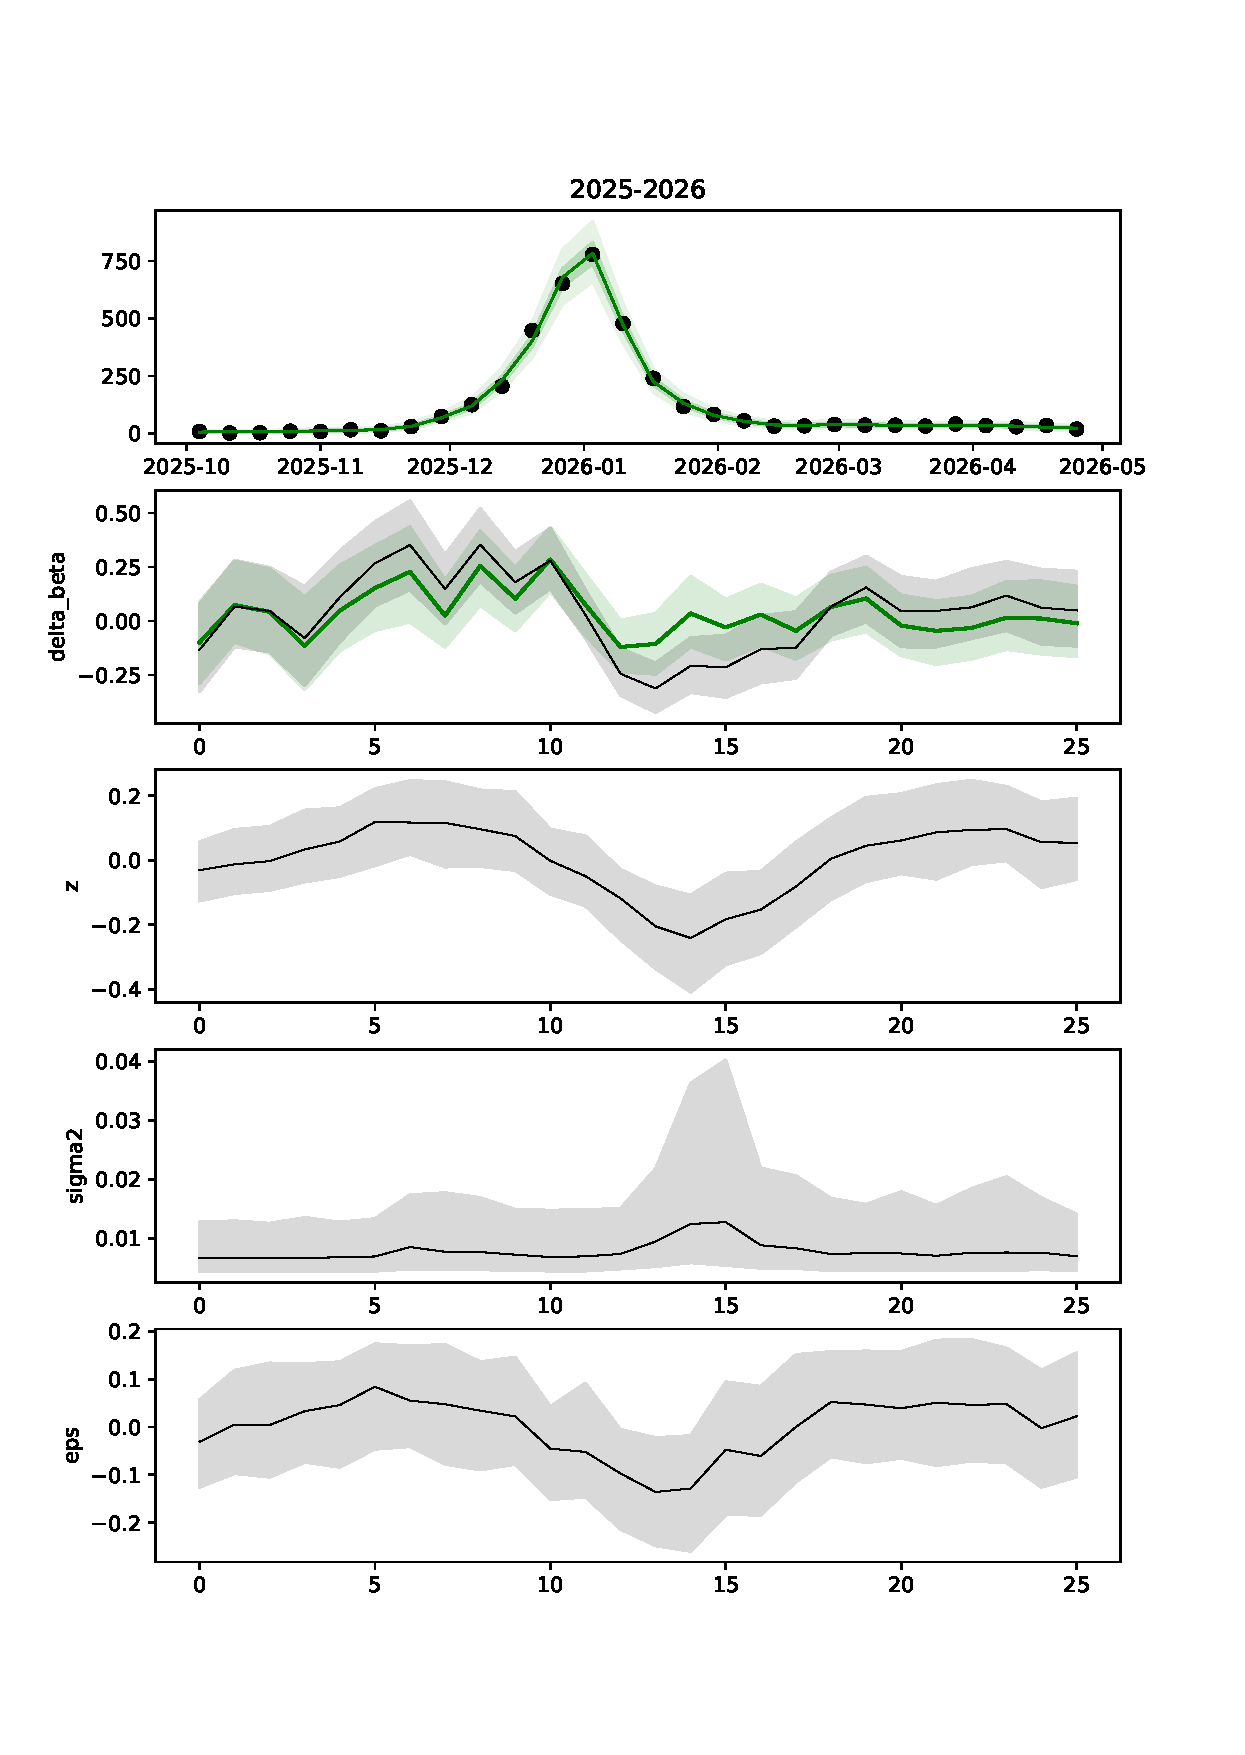
\includegraphics[width=0.85\linewidth]{fig/CT_2025-2026_goodness-fit.pdf}
    \caption{\textbf{Goodness-of-fit for Connecticut in the 2025--2026 season.} Observed number of influenza hospital admissions shown with markers, with the model's fit overlaid in green (first panel). Transmission modifiers $\Delta \mathcal{B}_{i,j}(l)$ in grey, and season mean modifiers $\Delta \mathcal{B}_j(l)$ in green (second panel). Deviation from the seasonal mean modifiers $z_{i,j}(l)$ (third panel). Volatility of the AR-GARCH system $\sigma_{i,j}(l)$ (fourth panel). Innovations of the AR-GARCH system $\epsilon_{i,j}(l)$ (fifth panel).}
    \label{fig:CT_2025-2026_goodness-fit}
\end{figure}

\begin{figure}[h!]
    \centering
    
\includegraphics[width=0.8\linewidth]{fig/forestplot-rho.pdf}
    \caption{\textbf{Posterior distribution of the ascertainment rate $\bm{\rho}$.} Distribution of the global effect $\bar{\rho}$ (top). Multiplicative state effects (bottom right). Multiplicative season effects (bottom left).}
    \label{fig:forestplot_rho}
\end{figure}

\begin{figure}[h!]
    \centering
    
\includegraphics[width=0.8\linewidth]{fig/forestplot-fI.pdf}
    \caption{\textbf{Posterior distribution of the initial fraction of infected individuals $\bm{f_I}$.} Distribution of the global effect $\bar{f}_I$ (top). Multiplicative state effects (bottom right). Multiplicative season effects (bottom left).}
    \label{fig:forestplot_fI}
\end{figure}

\begin{figure}[h!]
    \centering
    
\includegraphics[width=0.8\linewidth]{fig/forestplot-fR.pdf}
    \caption{\textbf{Posterior distribution of the initial fraction of recovered individuals $\bm{f_R}$.} Distribution of the global effect $\bar{f}_R$ (top). Odds-ratio of state effects (bottom right). Odds-ratio of season effects (bottom left).}
    \label{fig:forestplot_fR}
\end{figure}

\begin{figure}[h!]
    \centering
    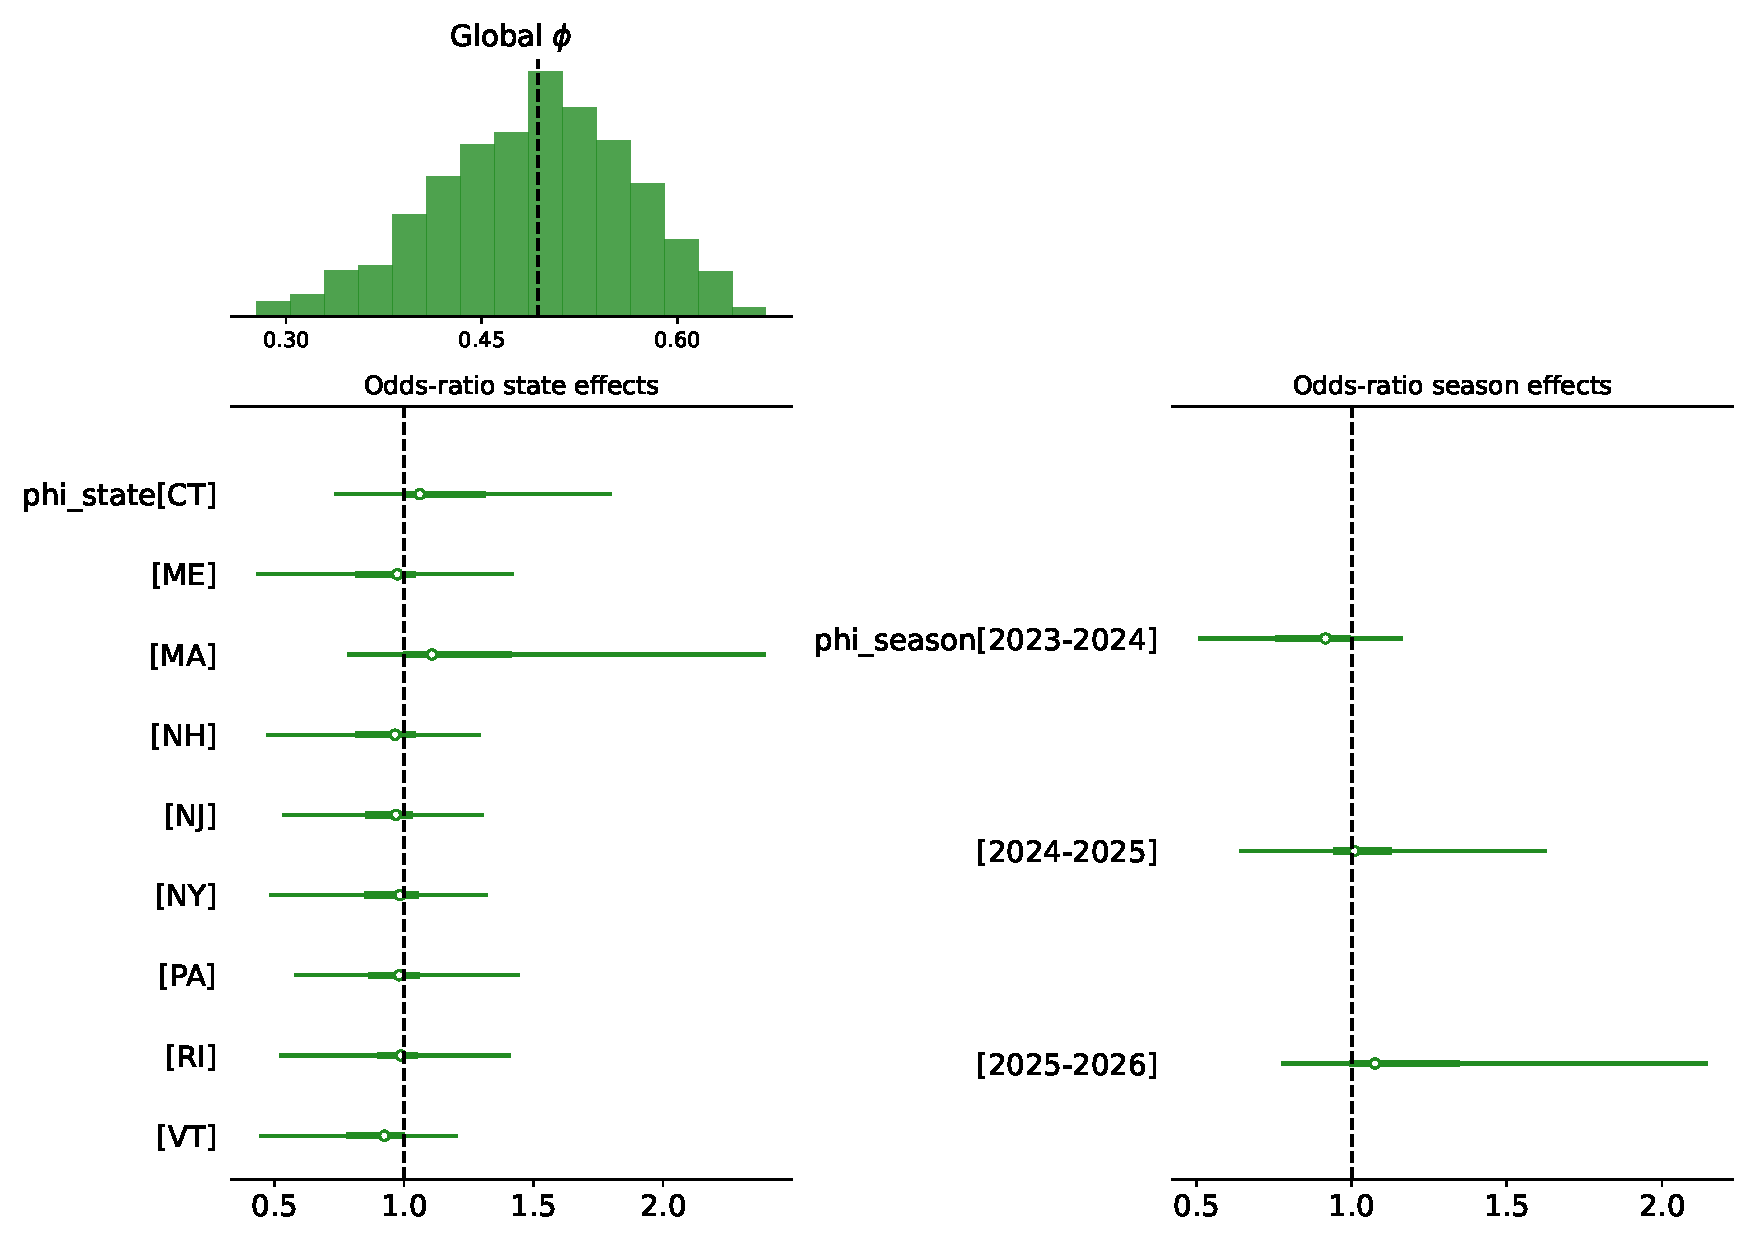
\includegraphics[width=0.8\linewidth]{fig/forestplot-phi.pdf}
    \caption{\textbf{Posterior distribution of the AR(1) persistence $\bm{\phi}$.} Distribution of the global effect $\bar{\phi}$ (top). Odds-ratio of state effects (bottom right). Odds-ratio of season effects (bottom left).}
    \label{fig:forestplot_phi}
\end{figure}

\begin{figure}[h!]
    \centering
    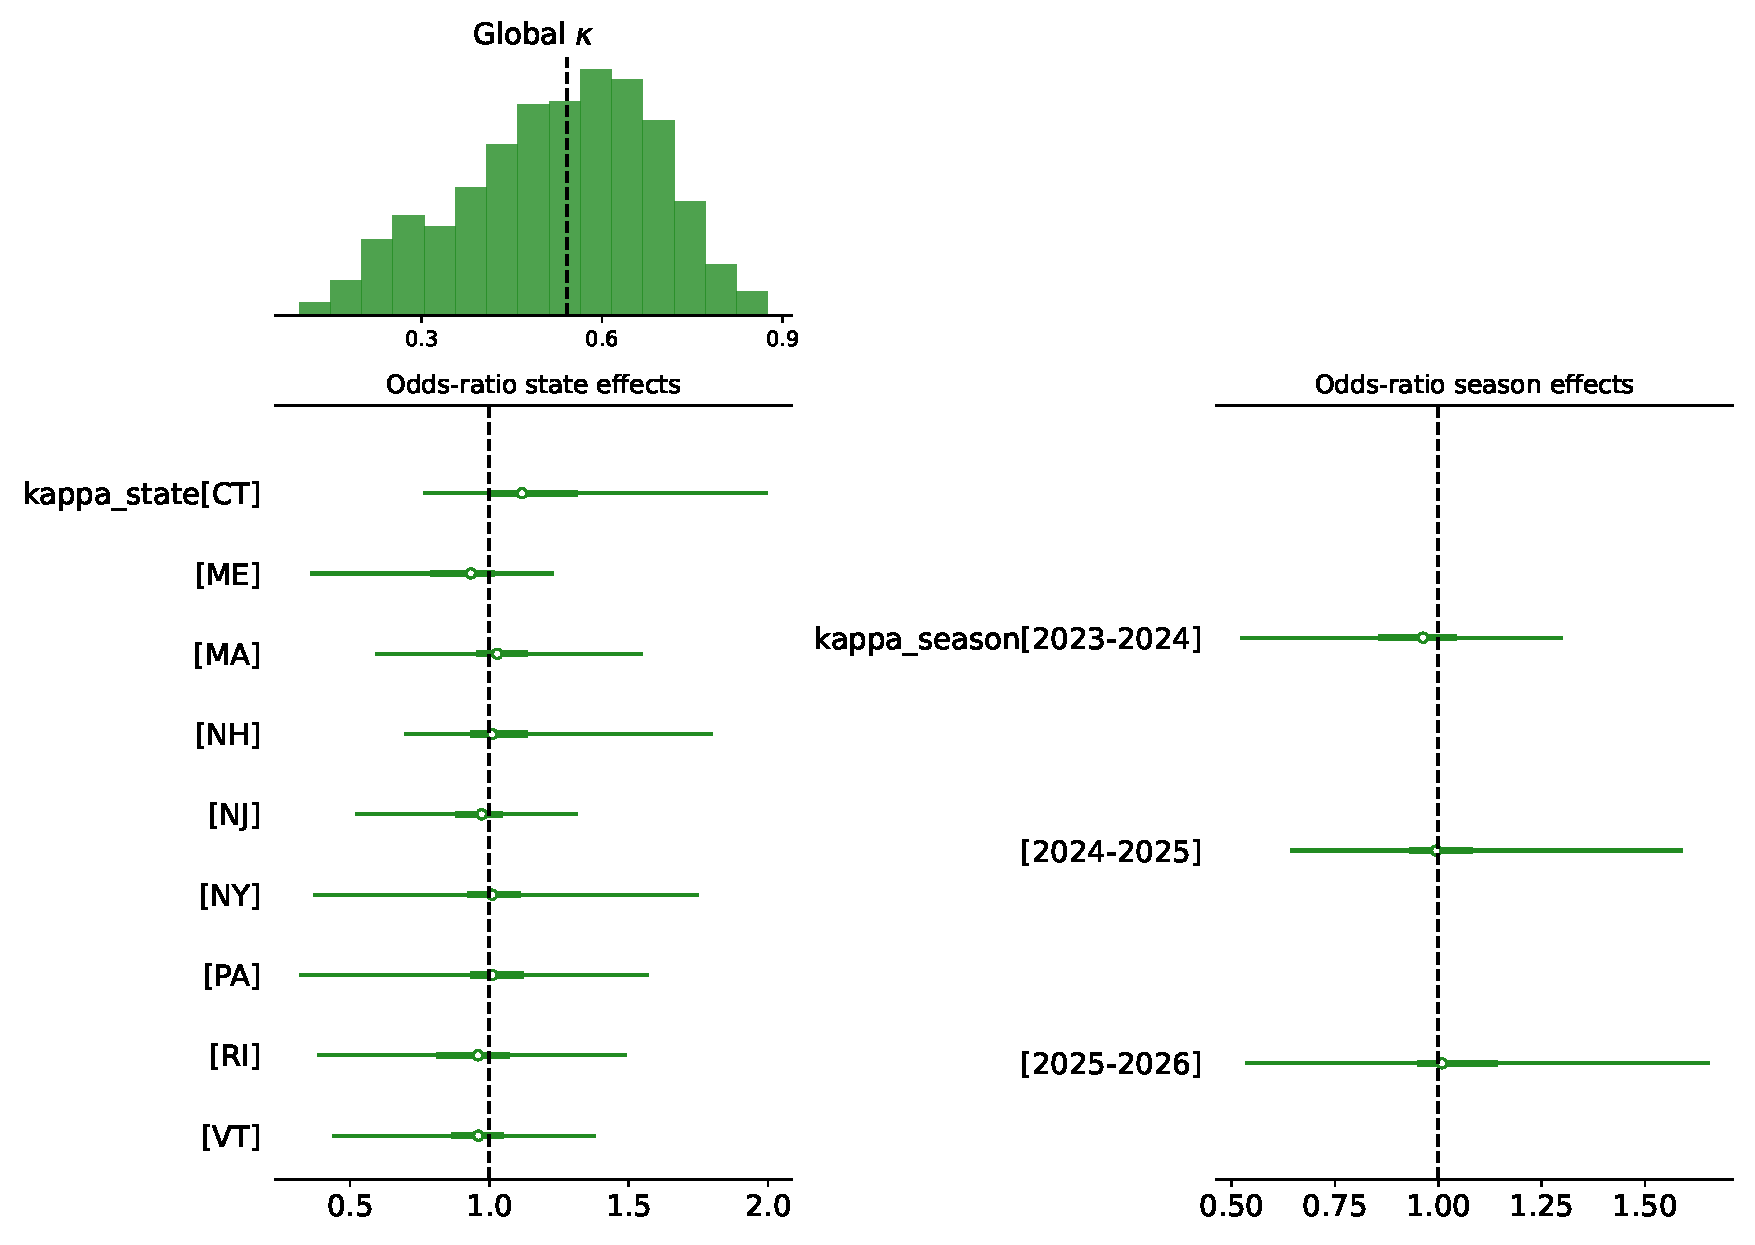
\includegraphics[width=\linewidth]{fig/forestplot-kappa.pdf}
    \caption{\textbf{Posterior distribution of the GARCH(1,1) total volatility persistence $\bm{\kappa}$.} Distribution of the global effect $\bar{\kappa}$ (top). Odds-ratio of state effects (bottom right). Odds-ratio of season effects (bottom left).}
    \label{fig:forestplot_kappa}
\end{figure}

\begin{figure}[h!]
    \centering
    
\includegraphics[width=\linewidth]{fig/trace-psi_1.pdf}
    \caption{\textbf{Traces of the spatial correlation of the seasonal mean modifiers $\bm{\psi_1}$.} Distribution (left). Sampled Markov chain (right).}
    \label{fig:trace_psi_1}
\end{figure}

\begin{figure}[h!]
    \centering
    
\includegraphics[width=\linewidth]{fig/trace-psi_2.pdf}
    \caption{\textbf{Traces of the spatial correlation of the stochastic deviations $\bm{\psi_2}$.} Distribution (left). Sampled Markov chain (right).}
    \label{fig:trace_psi_2}
\end{figure}

%-----------------------------------------------------------
\bibliographystyle{plainnat}
\bibliography{references}
%-----------------------------------------------------------

\end{document}